\documentclass{beamer}

\usepackage[utf8]{inputenc}
\usecolortheme{beaver}
\usepackage{caption}
\usepackage{subcaption}
\usepackage{mathtools}
\usepackage{todonotes}
\usepackage{amsmath}
\usepackage{bm}
\usepackage{listings}
\usepackage{ragged2e}
\usepackage{titlecaps}
\usepackage{fancyvrb}

\def\ci{\perp\!\!\!\!\!\perp}

\newtheorem{proposition}{Proposition}
\Addlcwords{for a is but and with of in as the etc on to if}

\setbeamertemplate{section in toc}{\inserttocsectionnumber.~\inserttocsection}
\usetheme{Boadilla}
\makeatletter
\setbeamertemplate{footline}{%
    \leavevmode%
    \hbox{%
        \begin{beamercolorbox}[wd=.3\paperwidth,ht=2.25ex,dp=1ex,center]{author in head/foot}%
            \usebeamerfont{author in head/foot}\insertshortauthor\expandafter\beamer@ifempty\expandafter{\beamer@shortinstitute}{}{~~(\insertshortinstitute)}
        \end{beamercolorbox}%
        \begin{beamercolorbox}[wd=.55\paperwidth,ht=2.25ex,dp=1ex,center]{title in head/foot}%
            \usebeamerfont{title in head/foot}\insertshorttitle
        \end{beamercolorbox}%
        \begin{beamercolorbox}[wd=.15\paperwidth,ht=2.25ex,dp=1ex,right]{date in head/foot}%
            \usebeamerfont{date in head/foot}\insertshortdate{}\hspace*{2em}
            \insertframenumber{} / \inserttotalframenumber\hspace*{2ex} 
        \end{beamercolorbox}}%
        \vskip0pt%
    }
\makeatother

\begin{document}

\title[]{Introduction to Casual Inference using pgmpy}
\date{}

\maketitle

\begin{frame}{Few real life examples}
	\begin{itemize}
		\item Finding how variables interact.
		\item Key drivers of an outcome.
	\end{itemize}
\end{frame}

\begin{frame}{Predictive vs Causal Questions}
\end{frame}

\begin{frame}{Frameworks for Causal Inference}
	\begin{itemize}
		\item Potential Outcomes Framework (Rubin's Causal Models): Use when you exactly know what you are trying to estimate.
			\begin{enumerate}
				\item Propensity score methods
				\item Doubly Robust Estimation
				\item Meta Learners: T-Learner, S-Learner, X-Learner.
			\end{enumerate}
		\item Directed Acyclic Graphs / Structural Causal Models: 
	\end{itemize}
\end{frame}

\begin{frame}{A General Workflow for Causal Inference}

\begin{figure}[t]
	\centering
	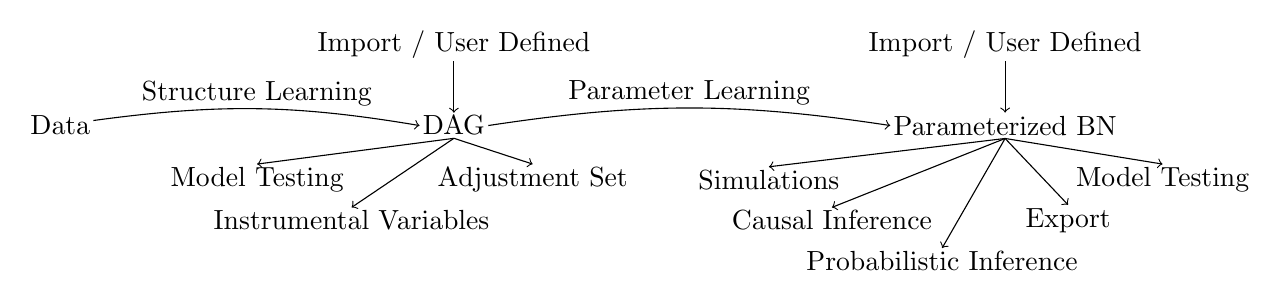
\begin{tikzpicture}[yscale=.86, inner sep=1pt]
	\tikzstyle{every node}=[align=left]
		\node (data)  at (0, 0) {Data};
		\node (dag)    at (5, 0) {DAG};
		\node (user)  at (5, 1.2) {Import / User Defined};
		\node (bn)    at (12, 0) {Parameterized BN};
		\node (test)  at (2.5, -0.8) {Model Testing};
		\node (iv)    at (3.7, -1.4) {Instrumental Variables};
		\node (as)    at (6, -0.8) {Adjustment Set};
		\node (sim)   at (9, -0.8) {Simulations};
		\node (ci)    at (9.8, -1.4) {Causal Inference};
		\node (pi)    at (11.2, -2) {Probabilistic Inference};
		\node (testp) at (14, -0.8) {Model Testing};
		\node (readwrite) at (12.8, -1.4) {Export};
		\node (read) at (12, 1.2) {Import / User Defined};

		\draw[->] (data) edge [bend left=10] node [midway, above]{Structure Learning} (dag.west);
		\draw (dag.east) edge [->,bend left=10] node [midway, above]{Parameter Learning} (bn.west);
		\draw[->] (user.south) -- (dag.north);
		\draw[->] (dag.south) -- (test.north);
		\draw[->] (dag.south) -- (iv.north);
		\draw[->] (dag.south) -- (as.north);
		\draw[->] (bn.south) -- (pi.north);
		\draw[->] (bn.south) -- (ci.north);
		\draw[->] (bn.south) -- (sim.north);
		\draw[->] (bn.south) -- (testp.north);
		\draw[->] (bn.south) -- (readwrite.north);
		\draw[->] (read.south) -- (bn.north);
	\end{tikzpicture}
	\caption{Possible workflows in pgmpy for Bayesian Networks}
	\label{fig:workflow}
\end{figure}

\end{frame}

\begin{frame}{Causal Discovery}
	\begin{itemize}
		\item How to get the DAG from the data?
		\item Usually the most challenging step of using the DAG framework.

		\item Really have to remember that: "All models are wrong, but some are useful" - George Box
		\item Many automated algorithms but most of them would make mistakes.
		\item Usually need to have some manual intervention. Need tools to guide this intervention.
		\item As the ground truth is not known, difficult to test how good our model is. Adhoc methods to help with it.
	\end{itemize}
\end{frame}

\begin{frame}{Integrating Expert Knowledge}
	\begin{itemize}
		\item Specify blacklisted/whitelisted edges.
		\item Specify starting model.
		\item Specify fixed edges.
	\end{itemize}
\end{frame}

\begin{frame}{Causal Discovery Algorithms learn a CPDAG}
	\begin{itemize}
		\item Trying to learn a network structure which matches the covariance
			structure.
		\item Multiple networks can represent the same casual structure.
		\item Structure learning algorithms usually a DAG.
	\end{itemize}

	Pairwise edge orientation rules.
\end{frame}

\begin{frame}
\end{frame}

\begin{frame}{LLM Based Structure Learning}

\end{frame}

\begin{frame}{Model evaluation}
	Lots of options for learning the models. How do know which one is the best?
	\begin{itemize}
		\item Implied CIs: Benefits, local testing, gives a hint of where things are wrong.
		\item Fisher C: Similar to implied CIs but summerizes the whole model fit.
		\item Compare models using likelihood or a scoring metric to see which fits better.
	\end{itemize}
\end{frame}

\begin{frame}{Using DAG in the PO framework}
	As DAGs explicitly show all the information, it can be used to make
	decisions in the PO framework as well.
\end{frame}

\begin{frame}{Identification}
	Second step: Assuming that we have an oriented DAG.
	Everything is identified in the case of fully observed models.

	When latent variables are present, need to determine identfiablity.
\end{frame}

\begin{frame}{do-calculus}
	\begin{itemize}
		\item Rules of do-calculus provide a full solution but no
			efficient algorithm.
		\item Other criterion with efficient algorithm but can only
			identify special cases.
		\item Back-door criterion
		\item Front-door criterion
		\item Instrumental variables.
	\end{itemize}
\end{frame}

\begin{frame}{pgmpy takes care of all this}
\end{frame}

\begin{frame}{Estimation}
	\begin{itemize}
		\item The identification method give the estimand.
		\item Use your favourite method for actual estimation.
	\end{itemize}
\end{frame}

\begin{frame}{Simulations}
\end{frame}

\begin{frame}{Lot more functionality}
	\begin{itemize}
		\item Other models such as SEM, Dynamic Bayesian Networks, Cluster Graphs.
		\item Probabilistic Inference
		\item Approximate Inference using Sampling
		\item Reading writing to interface with other packages.
		\item Plotting functionality
		\item Parameter Estimation
	\end{itemize}
\end{frame}

\begin{frame}
	Thank you.

	Consulting Company: Squanch Labs. Feel free to reach out to discuss use cases etc.
\end{frame}

\begin{frame}{Extra slide}
	When to use PO vs DAG framework?
\end{frame}

\begin{frame}
	How does it compare to Shapley values 
	\begin{itemize}
		\item Still prediction based. Does not matter if perturbing direct effect variable or undirect.
		\item Can show an example where Shapley values would still find an association, but causal inference would not. The standard confounding case.
	\end{itemize}
\end{frame}

\end{document}
